\appendix
\onecolumn
\begin{center}
\textbf{\Large Unsupervised Monocular Depth Estimation Using Atrous Convolutions}
\textbf{\large Supplementary Material}
\end{center}

\setcounter{figure}{0}
\renewcommand\thefigure{\thesection.\arabic{figure}}
\setcounter{table}{0}
\renewcommand{\thetable}{\thesection.\arabic{table}}

\section{Atrous Convolutions in the Encoder}\label{appendix:atrous-encoder}
\setcounter{figure}{0}  
    
    \begin{figure}[ht]
    \centering
    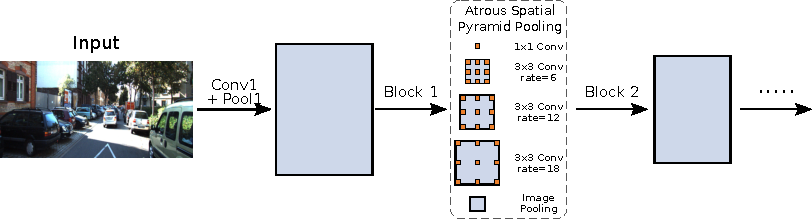
\includegraphics[width=0.8\textwidth]{images/architecture/aspp-in-encoder.pdf}
    \caption{ASPP after the first ResNet block.}
    \label{fig:appendix:aspp-encoder}
    \end{figure}
    \begin{figure}[ht]
    \centering
    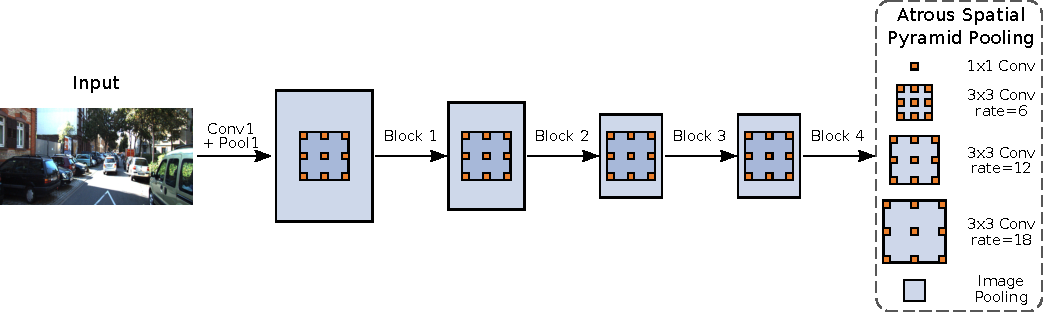
\includegraphics[width=0.8\textwidth]{images/architecture/encoder-with-atrous-rates.pdf}
    \caption{Atrous convolutions inside the ResNet blocks.}
    \label{fig:appendix:resnet-atrous}
    \end{figure}
    
     
\section{Reconstruction error plots}
\setcounter{figure}{0}    
% the \\ insures the section title is centered below the phrase: AppendixA

\begin{figure}[h!]
\centering
\begin{subfigure}[c]{0.24\textwidth}
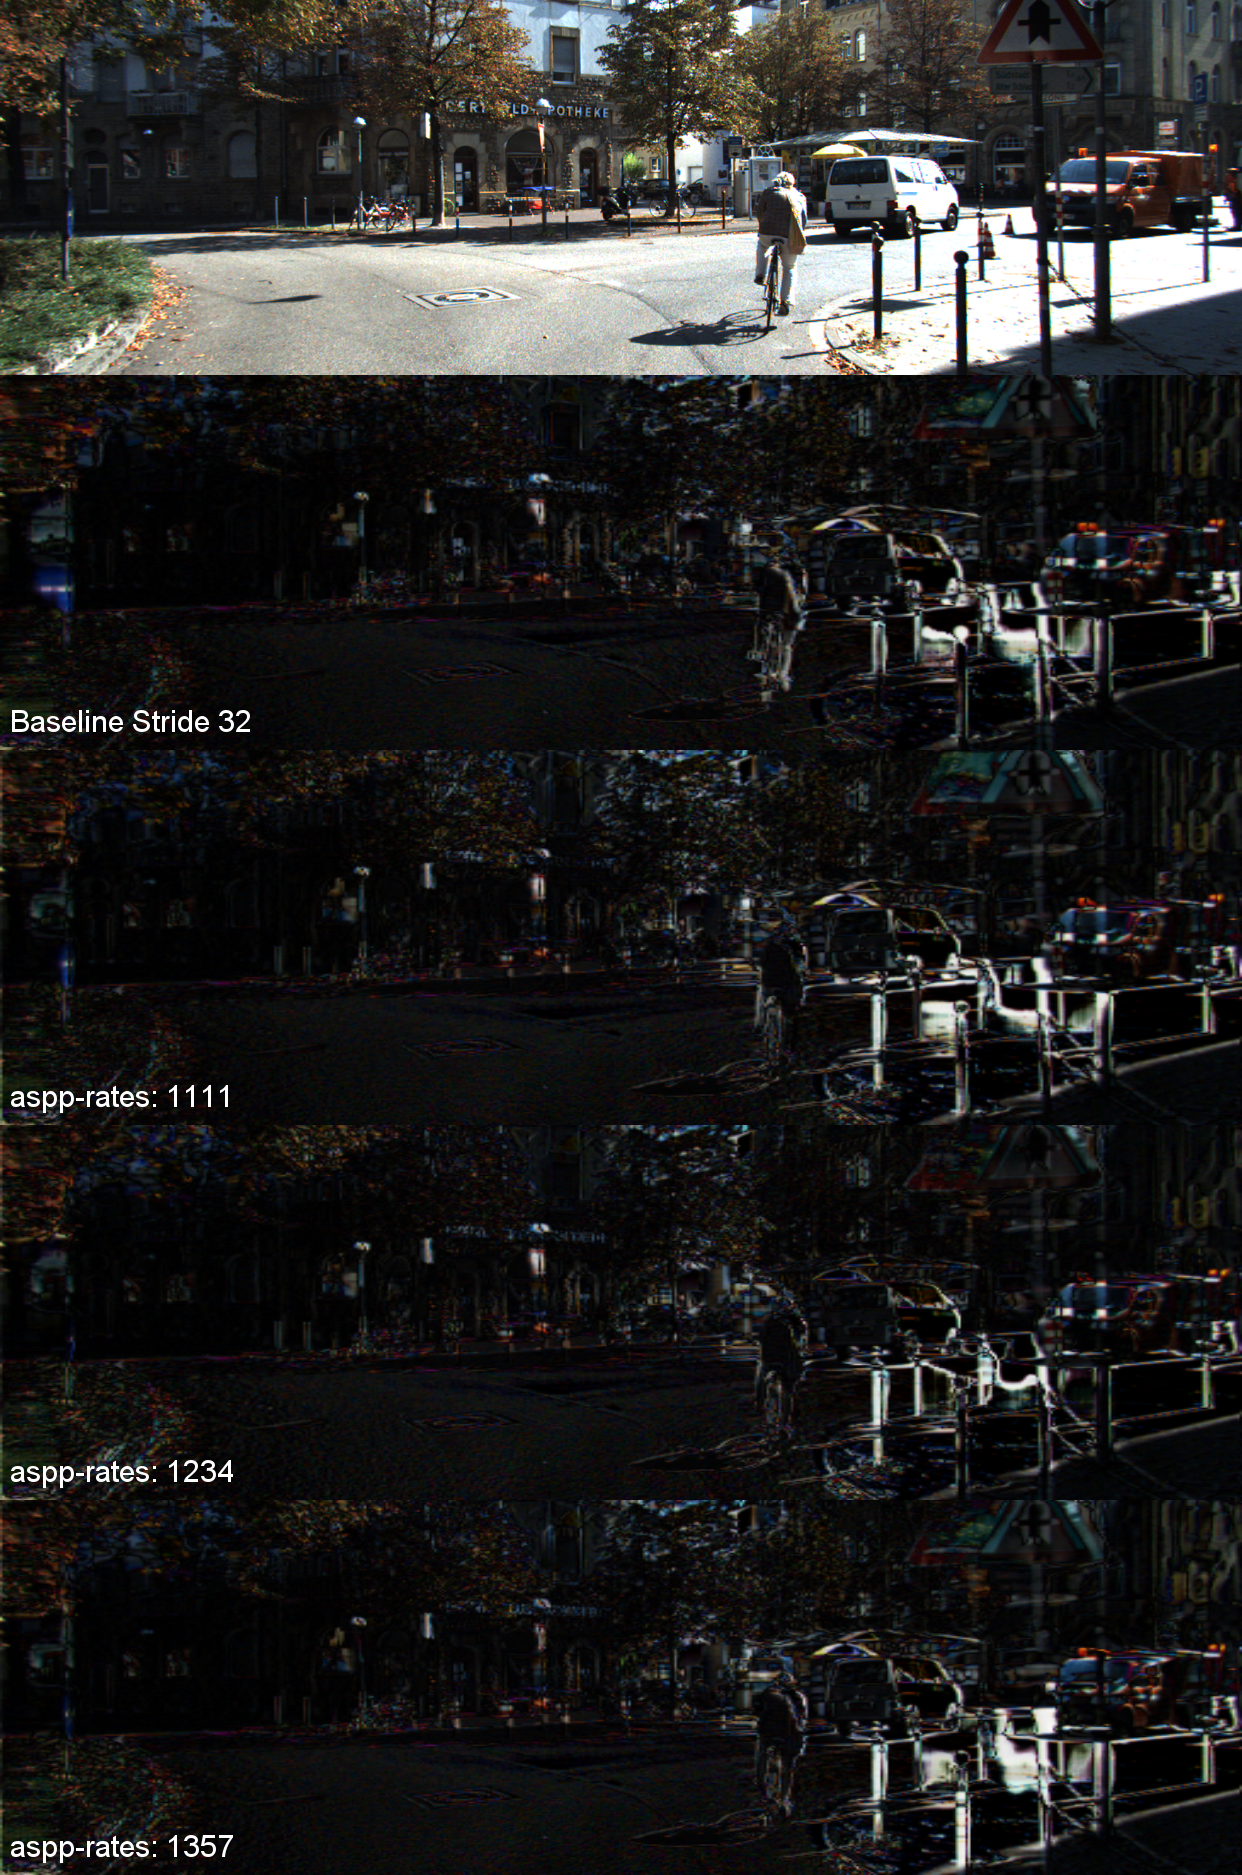
\includegraphics[width=\textwidth]{images/visual_comparisons/reconstruction_error/concat_003.png}
\end{subfigure}
\begin{subfigure}[c]{0.24\textwidth}
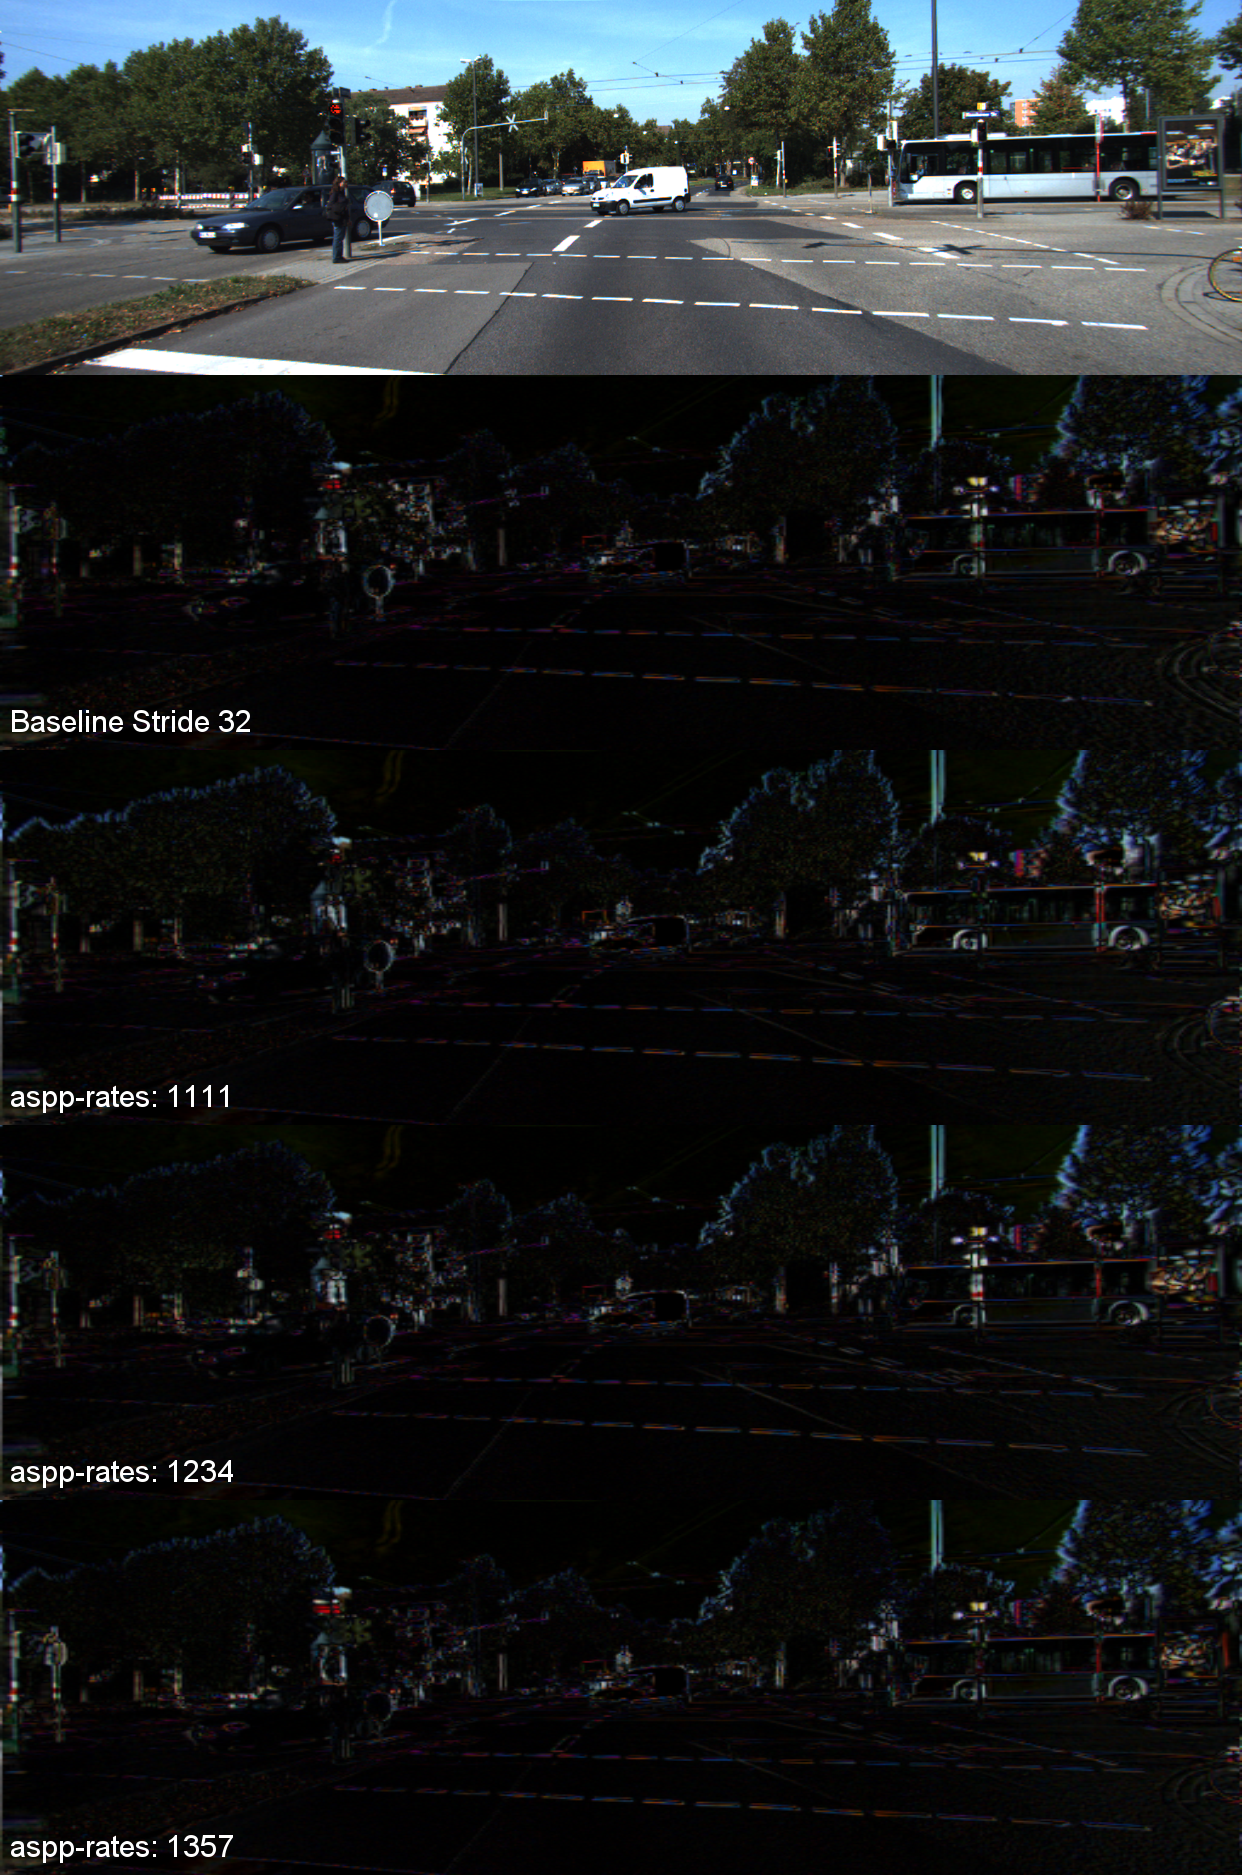
\includegraphics[width=\textwidth]{images/visual_comparisons/reconstruction_error/concat_015.png}
\end{subfigure}
\begin{subfigure}[c]{0.24\textwidth}
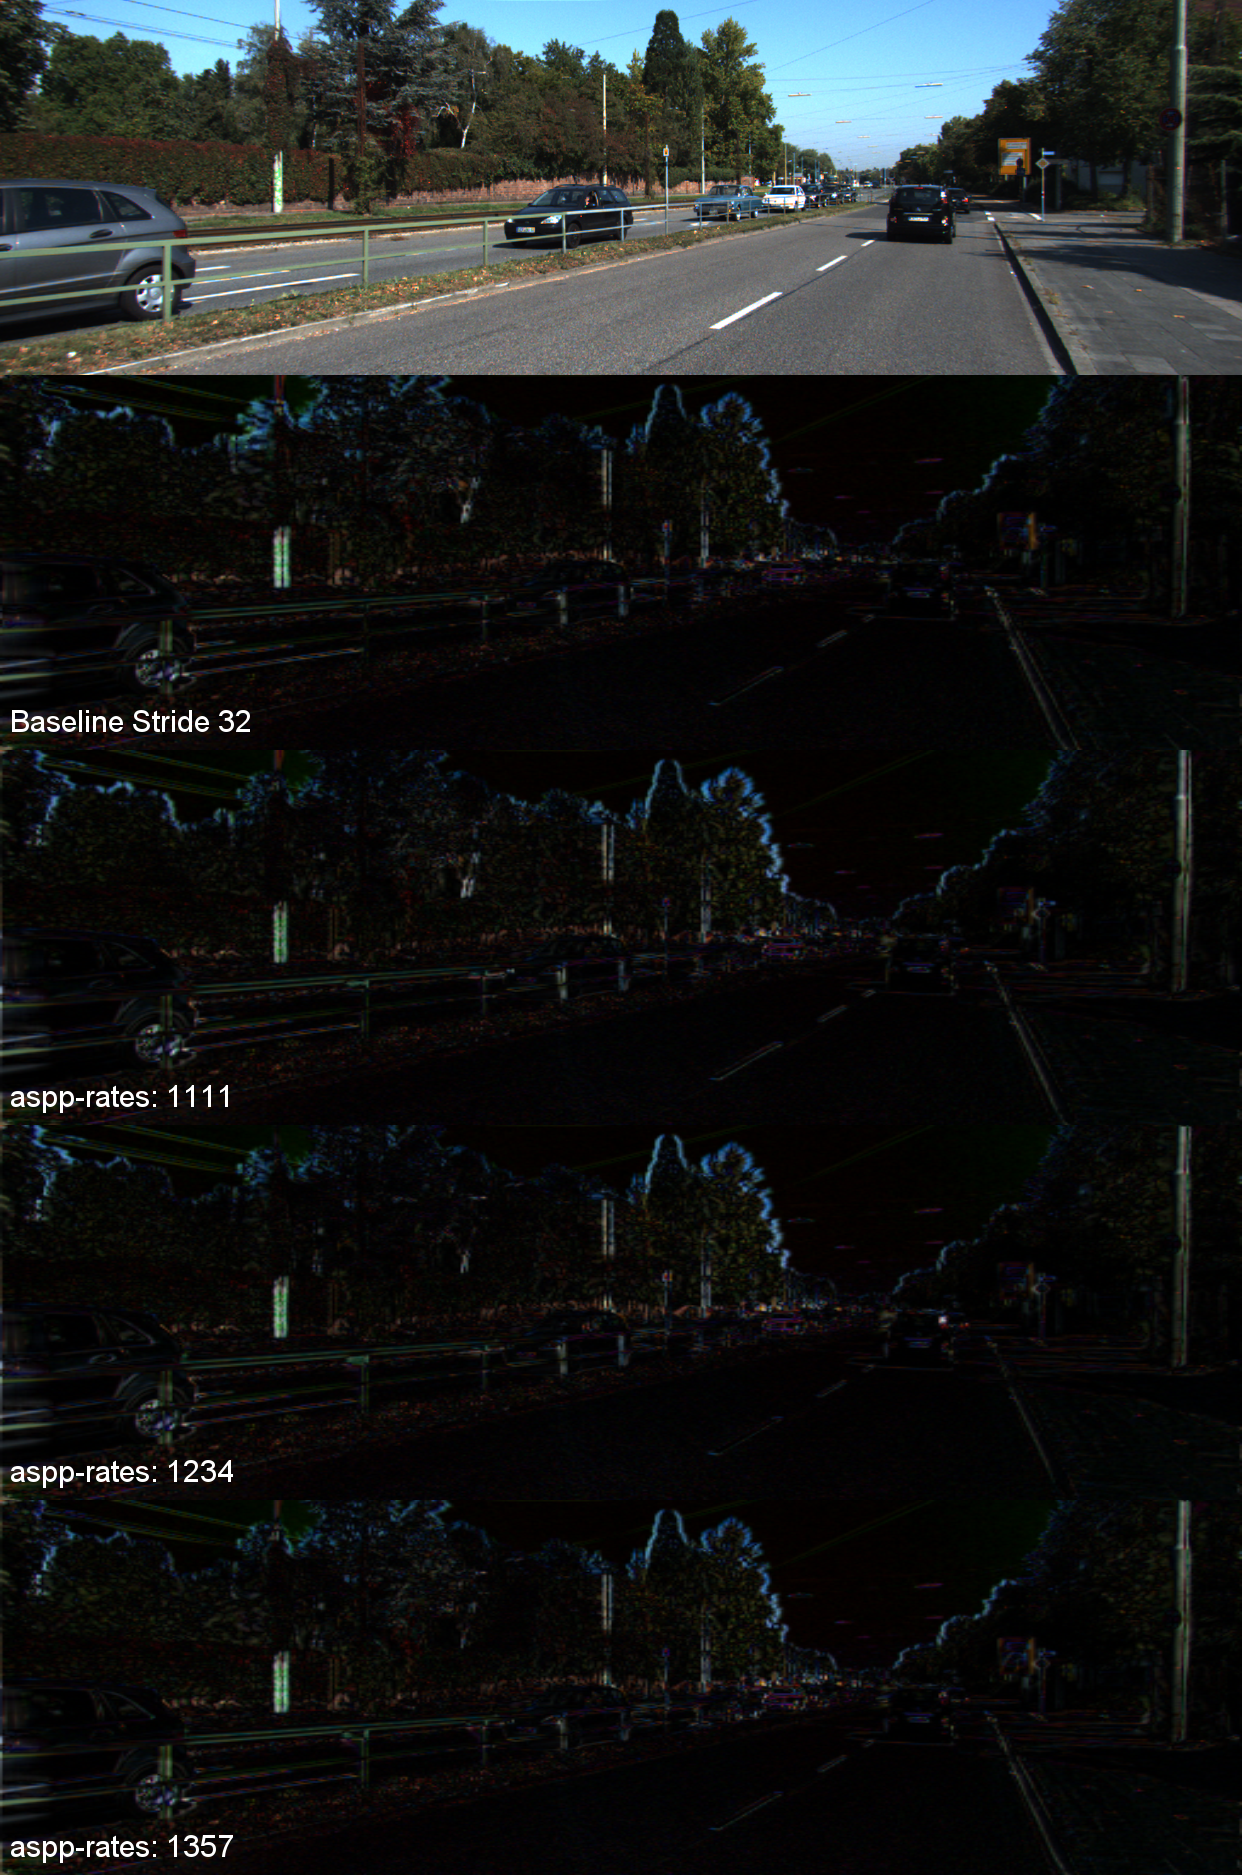
\includegraphics[width=\textwidth]{images/visual_comparisons/reconstruction_error/concat_024.png}
\end{subfigure}
\begin{subfigure}[c]{0.24\textwidth}
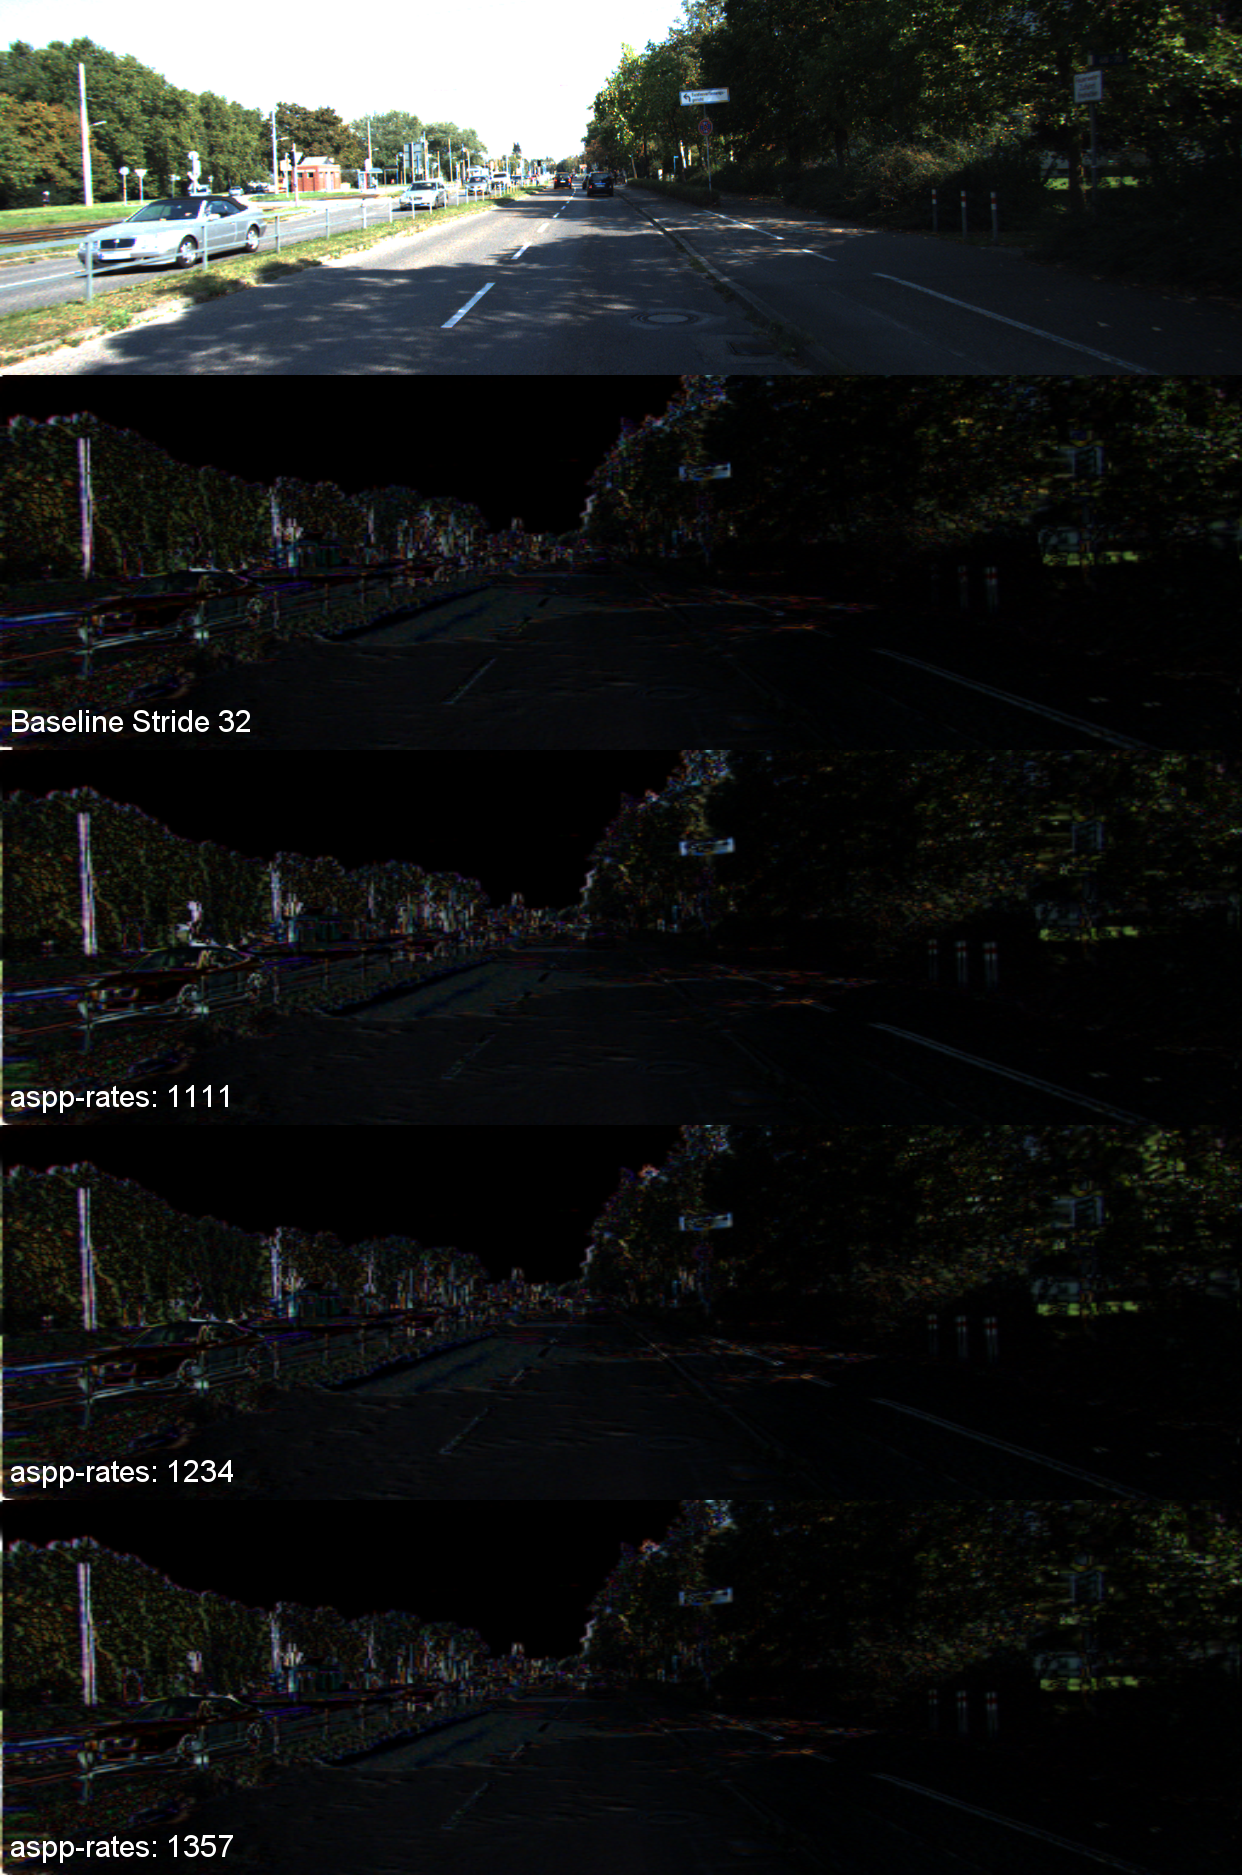
\includegraphics[width=\textwidth]{images/visual_comparisons/reconstruction_error/concat_029.png}
\end{subfigure}
\caption{Reconstruction error for the experiment in Section \ref{section:aspp-rates} in which the impact of different atrous rates ([1,1,1,1], [1,2,3,4], [1,3,5,7]) was compared to the baseline.}
\label{appendix:reconstruction-error}
\end{figure}

\section{VKITTI Error Maps}
\begin{figure}[h!]
\centering
\begin{subfigure}[c]{0.24\textwidth}
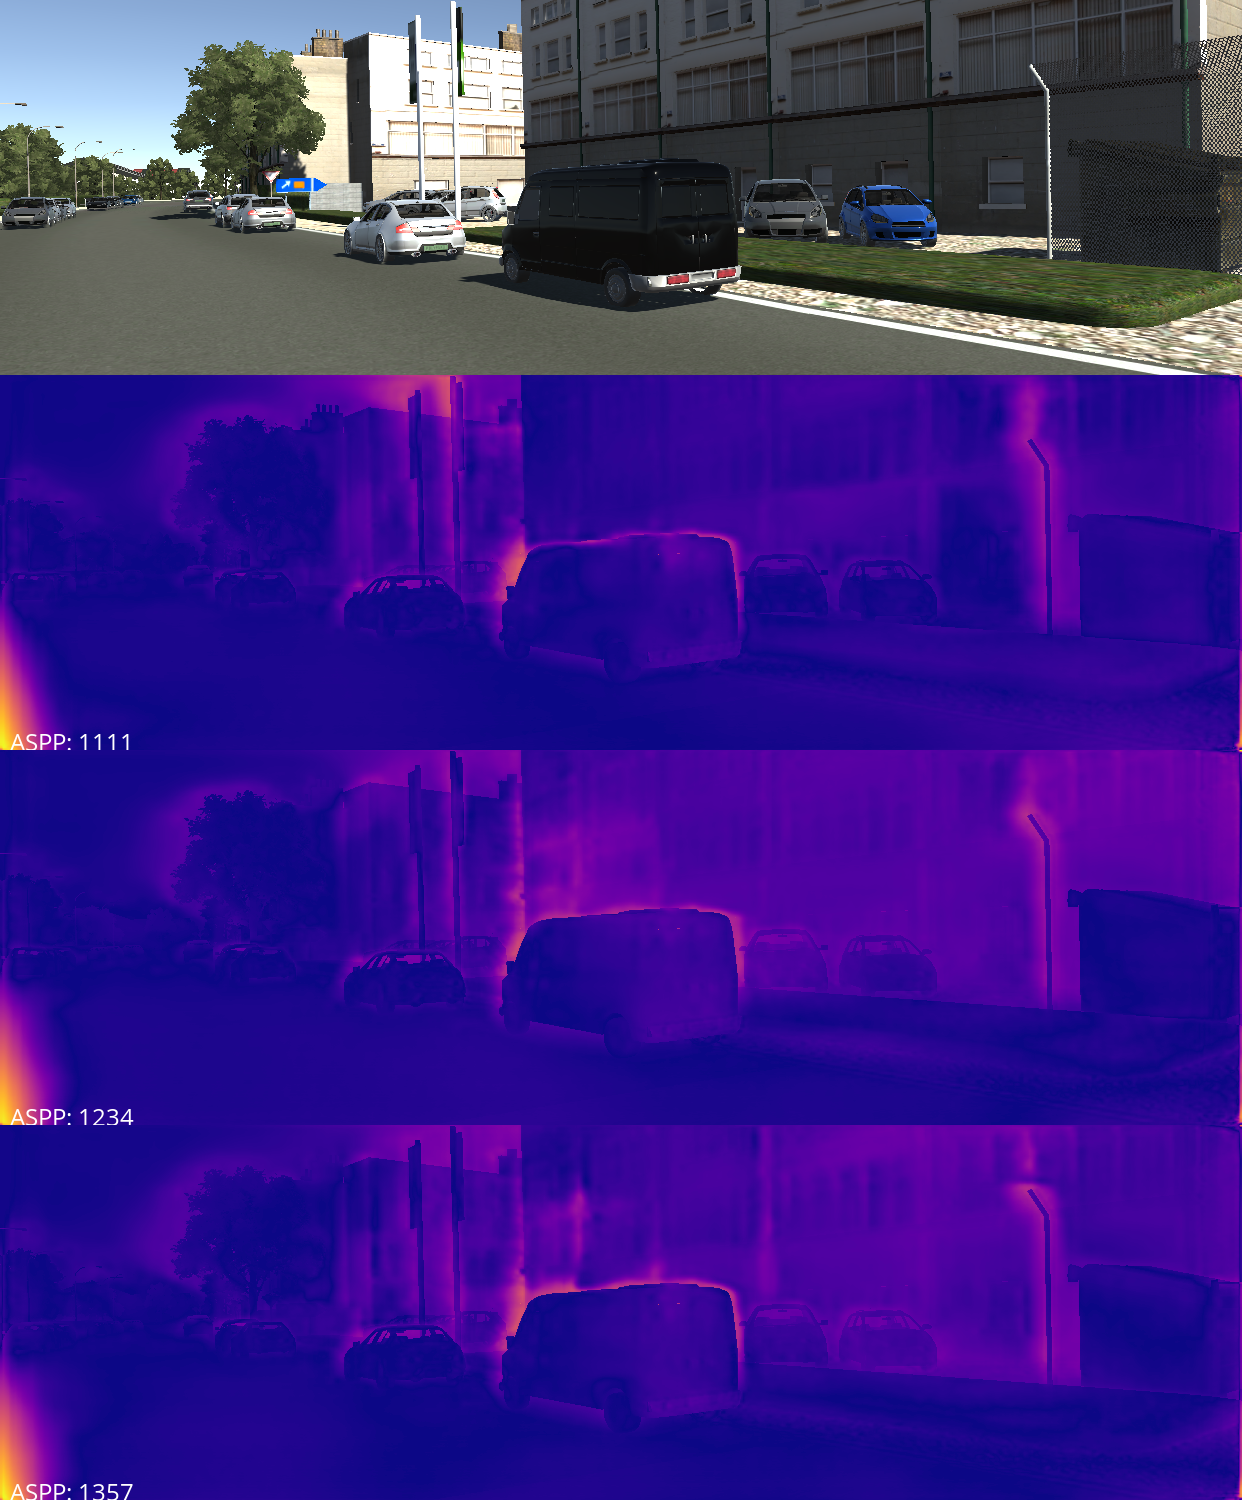
\includegraphics[width=\textwidth]{images/visual_comparisons/aspp-rates-vkitti/concat_221.png}
\end{subfigure}
\begin{subfigure}[c]{0.24\textwidth}
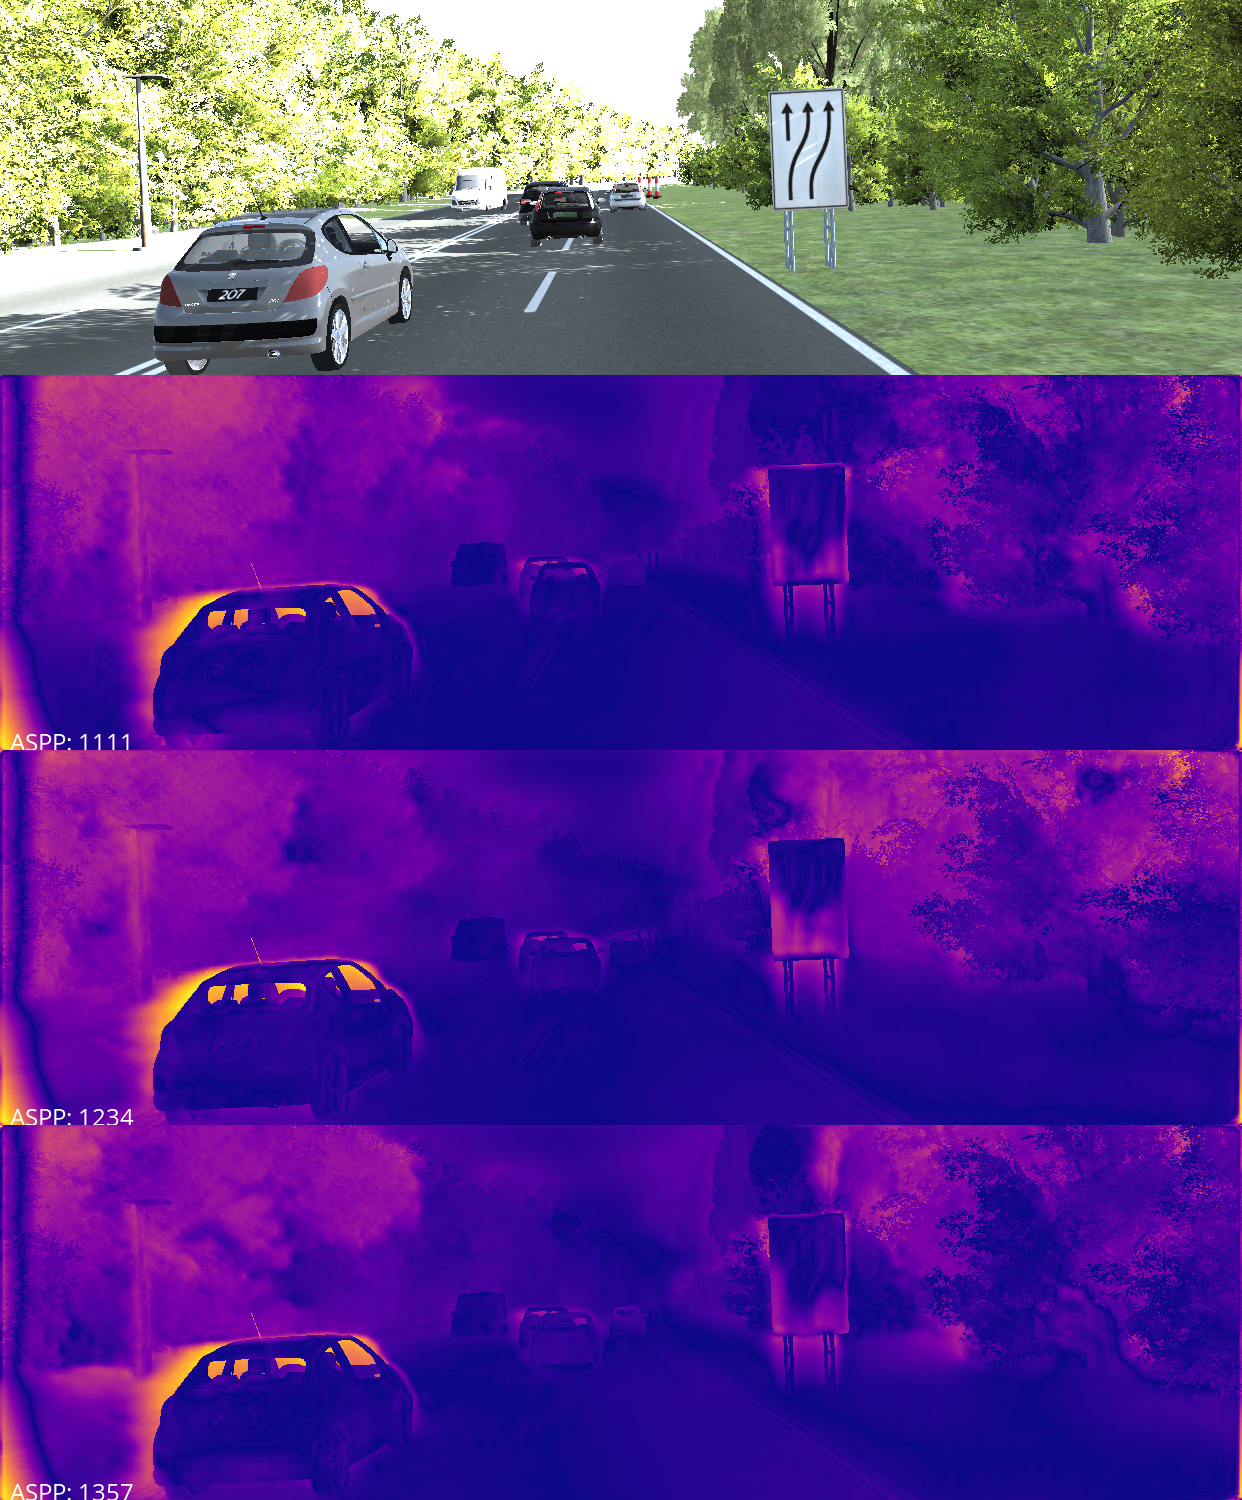
\includegraphics[width=\textwidth]{images/visual_comparisons/aspp-rates-vkitti/concat_1226.png}
\end{subfigure}
\begin{subfigure}[c]{0.24\textwidth}
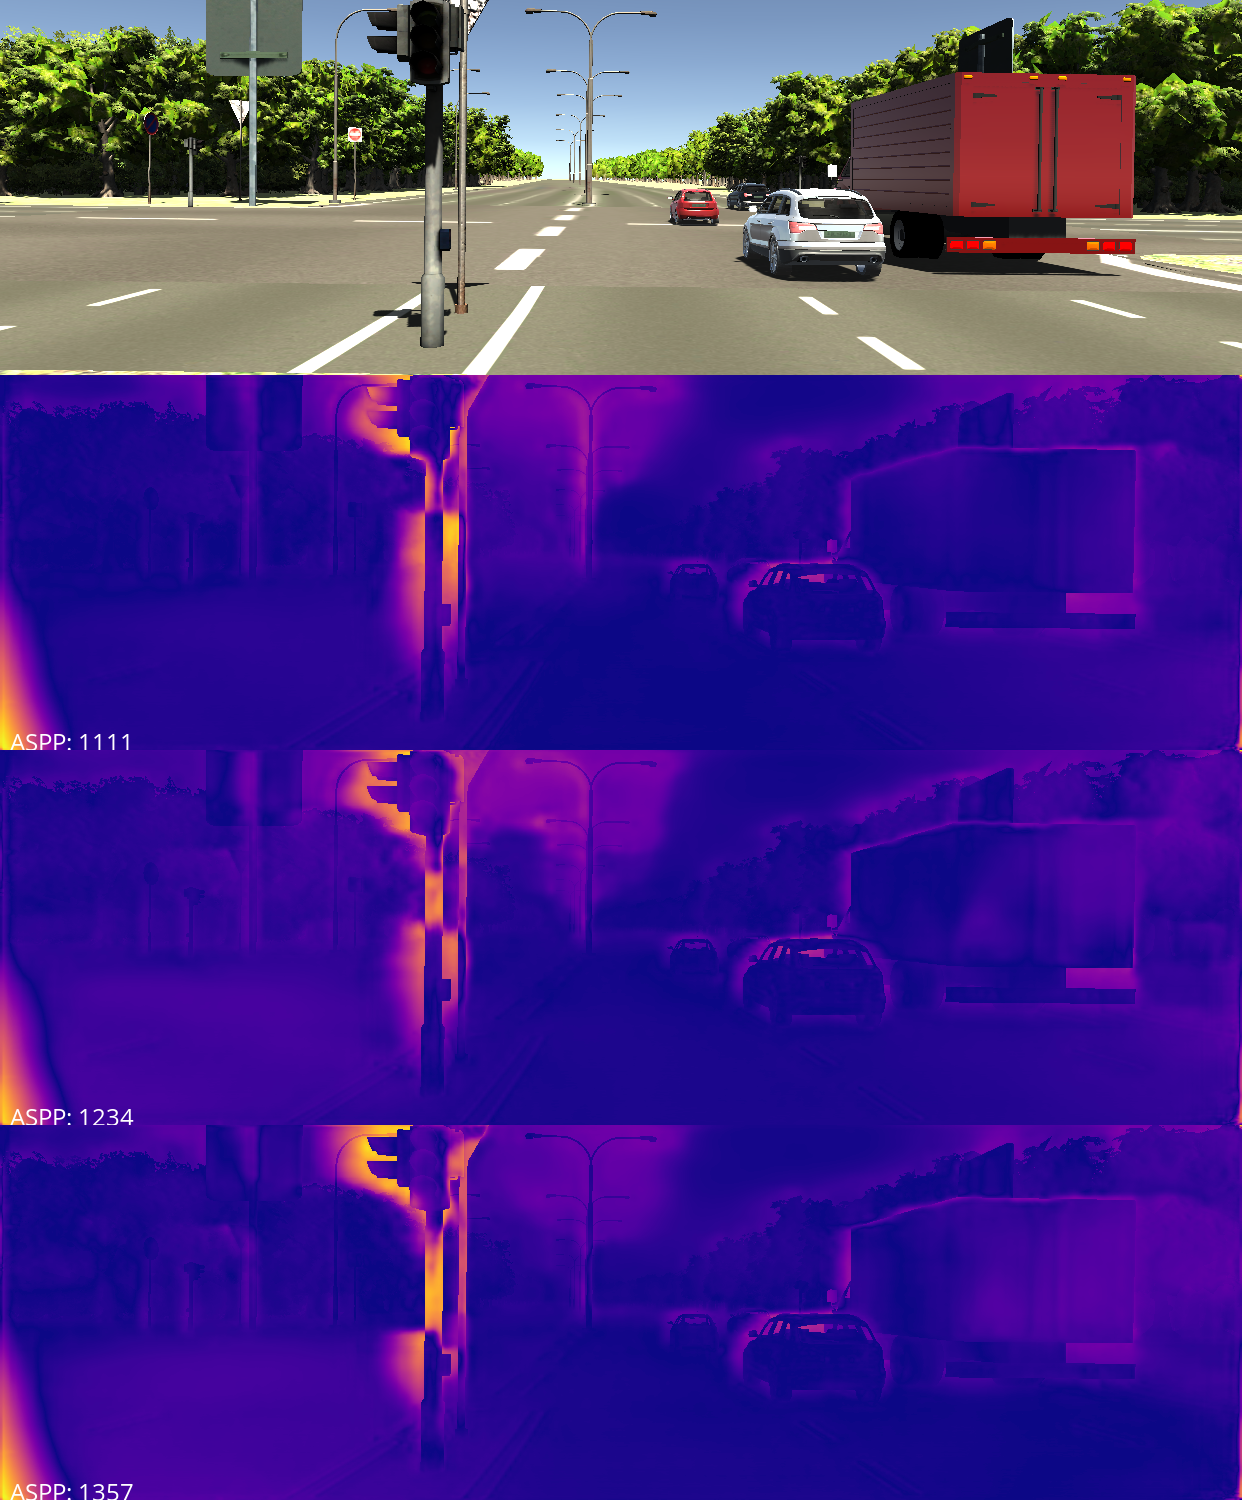
\includegraphics[width=\textwidth]{images/visual_comparisons/aspp-rates-vkitti/concat_763.png}
\end{subfigure}
\begin{subfigure}[c]{0.24\textwidth}
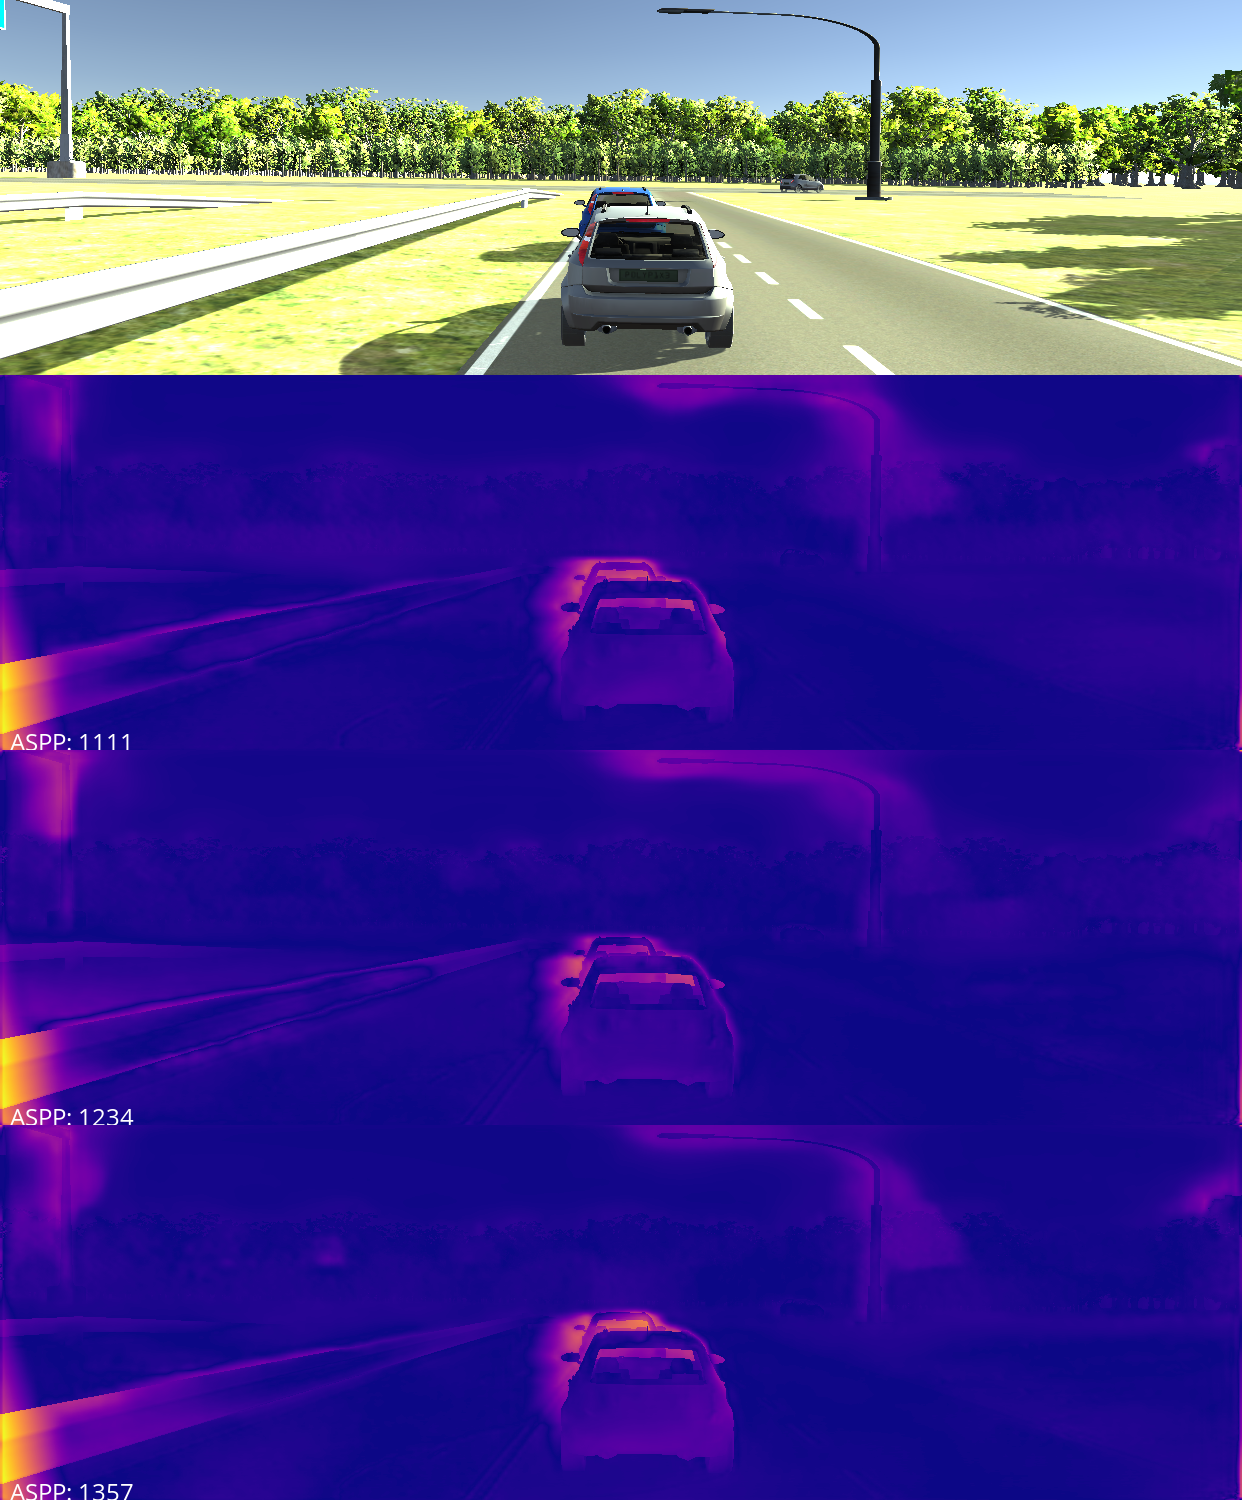
\includegraphics[width=\textwidth]{images/visual_comparisons/aspp-rates-vkitti/concat_2083.png}
\end{subfigure}
\caption{Disparity error maps on VKITTI (cf. Section \ref{section:vkitti}), in which the impact of different atrous rates ([1,1,1,1], [1,2,3,4], [1,3,5,7]) are compared.}
\label{fig:appendix:vkitti}
\end{figure}


\section{Full Experimental Results}\label{appendix:full-results}
\setcounter{figure}{0}    
% the \\ insures the section title is centered below the phrase: Appendix B


\begin{table}[ht]
    \centering
    \begin{tabular}{lllrrrrrrrrr}
    \toprule
     Output-stride & Abs.Rel. &  Sq.Rel. &   RMSE &  Log RMSE &     $\delta < 1.25^1$ &     $\delta < 1.25^2$ &     $\delta < 1.25^3$ &      Params (M) \\
    \midrule 
           8   &   0.1068  &  1.0408  &  5.533  &  0.197  &  0.859  &  0.946  &  0.979 & 58.4\\
           16  &   0.1041  &  1.0097  &  5.362  &  0.191  &  0.865  &  0.951  &  0.981 & 58.4\\
           32  &   0.1048  &  1.0353  &  5.458  &  0.191  &  0.866  &  0.949  &  0.980 & 58.4\\
           64  &   0.1120  &  1.2025  &  5.716  &  0.201  &  0.854  &  0.948  &  0.981 & 58.4\\
    \bottomrule
    \end{tabular}
    \caption{Comparison of output stride 8, 16, 32 and 64.}
\end{table}


\begin{table}[ht]
    \centering
    \begin{tabular}{lllrrrrrrrrr}
    \toprule
     Output-stride & ASPP &  Abs.Rel. &  Sq.Rel. &   RMSE &  Log RMSE &     $\delta < 1.25^1$ &     $\delta < 1.25^2$ &     $\delta < 1.25^3$ &      Params (M) \\
    \midrule 
           16  &  1-1-1-1 &   0.1007  &  0.9439  &  5.322  &  0.186  &  0.871  &  0.956  &  0.983 & 58.4\\
           16  &  1-2-3-4 &   0.1038  &  0.9571  &  5.351  &  0.187  &  0.867  &  0.956  &  0.980 & 58.4\\
           16  &  1-3-5-7 &   0.1058  &  0.9803  &  5.472  &  0.192  &  0.864  &  0.95-  &  0.981 & 58.4 \\
           \addlinespace
           32  &  1-1-1-1 &   0.1021  &  0.9561  &  5.300  &  0.185  &  0.870  &  0.956  &  0.984 & 58.4 \\
           32  &  1-2-3-4 &   0.1037  &  1.0007  &  5.446  &  0.190  &  0.869  &  0.954  &  0.983 & 58.4 \\
           32  &  1-3-5-7 &   0.1055  &  1.0374  &  5.421  &  0.191  &  0.866  &  0.951  &  0.982 & 58.4 \\
    \bottomrule
    \end{tabular}
    \caption{Experiment on the influence of increasing atrous rates in the ASPP block for output stride 16 and 32. For both output strides, increasing the atrous rates has increased the depth estimation error on all metrics.}
\end{table}


\begin{table}[ht]
    \centering
    \setlength{\tabcolsep}{4pt}
    \begin{tabular}{lllrrrrrrrrr}
    \toprule
     Output-stride & ASPP &  Abs.Rel. &  Sq.Rel. &   RMSE &  Log RMSE &     $\delta < 1.25^1$ &     $\delta < 1.25^2$ &     $\delta < 1.25^3$ &      Params (M) \\
    \midrule 
           32  &  1             &   0.1036  &  1.0123  &  5.403  &  0.187  &  0.867  &  0.955  &  0.984 & 44.1 \\
           32  &  1-1           &   0.1027  &  1.0260  &  5.373  &  0.188  &  0.872  &  0.955  &  0.983 & 48.9 \\
           32  &  1-1-1         &   0.1020  &  0.9639  &  5.356  &  0.188  &  0.868  &  0.956  &  0.983 & 53.6 \\
           32  &  1-1-1-1       &   0.1021  &  0.9561  &  5.300  &  0.185  &  0.870  &  0.956  &  0.984 & 58.4 \\
           32  &  1-1-1-1-1     &   0.1014  &  0.9703  &  5.303  &  0.186  &  0.873  &  0.955  &  0.984 & 63.3 \\
           32  &  1-1-1-1-1-1   &   0.1024  &  0.9893  &  5.419  &  0.189  &  0.868  &  0.954  &  0.982 & 68.0 \\
           32  &  1-1-1-1-1-1-1 &   0.1025  &  0.9820  &  5.341  &  0.869 &  0.957  &  0.984  &  0.983 & 72.8 \\
    \bottomrule
    \end{tabular}
    \caption{Number of ASPP Modules. The evaluation results become better the more parallel convolutions are used in the ASPP. The point of diminishing returns is reached after about 7 convolutions. The number of parameters increases by about 4.8 million for each additional convolution.}
\end{table}


\begin{table}[ht]
    \centering
    \begin{tabular}{lllrrrrrrrrr}
    \toprule
     Output-stride & ASPP &  Abs.Rel. &  Sq.Rel. &   RMSE &  Log RMSE &     $\delta < 1.25^1$ &     $\delta < 1.25^2$ &     $\delta < 1.25^3$ &      Params (M)\\
    \midrule 
           32  &  1-1-1-1 &   0.1065 &     1.0612 &     5.519 &      0.194 &      0.861 &      0.951 &      0.982 & 60.7\\
           32  &  1-6-12-18 &   0.1108 &     1.1424 &      5.615 &      0.197 &      0.858 &      0.947 &      0.980 & 60.7\\
    \bottomrule
    \end{tabular}
    \caption{ASPP after the first ResNet block. The model with only standard (\textit{atrous rate} $=1$) convolutions performed better.}
    \label{table:appendix:aspp-encoder}
\end{table}


\begin{table}[h]
    \centering
    \begin{tabular}{lllrrrrrrrrr}
    \toprule
     Output-stride & Atrous rates &  Abs.Rel. &  Sq.Rel. &   RMSE &  Log RMSE &     $\delta < 1.25^1$ &     $\delta < 1.25^2$ &     $\delta < 1.25^3$ &      Params (M)\\
    \midrule 
           16  &  1-1-1-1 &   0.1007 &     0.9439 &      5.322 &      0.186 &      0.871 &      0.956 &      0.983 & 58.4\\
           16  &  1-2-1-2 &   0.1028 &     0.9788 &      5.360 &      0.188 &      0.867 &      0.954 &      0.983 & 58.4\\
    \addlinespace
           64  &  1-1-1-2 &  0.1110 &     1.0958 &      5.627 &      0.197 &      0.857 &      0.949 &      0.981 & 58.4\\
           64  &  1-2-1-2 &  0.1135 &     1.1240 &      5.675 &      0.200 &      0.851 &      0.947 &      0.980 & 58.4\\
    \bottomrule
    \end{tabular}
    \caption{Atrous convolutions inside the ResNet blocks. This experiment was conducted two different output strides (64 and 16). We changed the atrous rates of the main convolutional layer in the four ResNet blocks. Less atrous convolutions lead to better numerical scores.}
    \label{table:appendix:atrous-encoder}
\end{table}